\chapter{INTRODUCTION}
\thispagestyle{fancy}
\pagenumbering{arabic}
\setcounter{page}{1}


	\section{Background} 
        		March of 2016 was a very exciting period for the machine learning community. Almost two
        decades after IBM's Deep Blue beat the world champion Garry Kasparov at chess, the field of AI was
        ready to take another board game from its checklist: Go. Lee Sedol, a professional Go player with
        the highest rank possible was challenged by Google DeepMind to compete against their AI program
        AlphaGo in a 5-game match of Go. While Lee Sedol was very confident of winning - \textit{"I dont think it will
        be a very close match. I believe it will be 5-0, or maybe 4-1. So the critical point for me will be to not lose one
        match."} \cite{leesedol}- AlphaGo managed to defeat him with a 4 to 1 score. Before this match, the game of Go
        was regarded as too hard for modern technology, because of the immense state-space. However, the
        DeepMind's team managed to defy all expectation by reaching this new milestone in modern AI. More
        specifically they did this by combining two very powerful machine learning techniques: deep learning
        and reinforcement learning. The combination of these techniques form the foundation of a new field in
        machine learning called \textit{deep reinforcement learning}.
        \par
        For decades it was impossible to perform machine learning techniques directly on an environment that's changing frequently (like video games). Until the breakthrough of deep learning in 2012 \cite{Krizhevsky:2012:ICD:2999134.2999257}, most of the techniques relied on handcrafted
        features. These handcrafted features need to be manually defined by researchers, showing which \textit{parts} or features from a dataset is important. Take the subfield of supervised learning that focuses on image recognition as an example. Before an image could be fed to a classification model like e.g. a support vector machine, it had to go through a manually
        designed feature extraction step, like deciding which part of the image is the main focus, doing edge detection,  or determining the graph representation of an alphabetic character. The success of the classification task mostly relied on the quality of the
        handcrafted features, which can be time-consuming to develop. The introduction of various deep learning techniques, made it possible to extract high-level features directly from raw inputs, without the need
        for human intervention. Simply, there's little to no predefined "things" in the agent, allowing the AI to be as general as possible. The technique revolutionized the field computer vision and speech recognition
        by drastically improving the performance on benchmarks in both fields. \cite{Krizhevsky:2012:ICD:2999134.2999257}\cite{DBLP:journals/corr/abs-1303-5778}.
                 \begin{figure}[H]
            \centering
            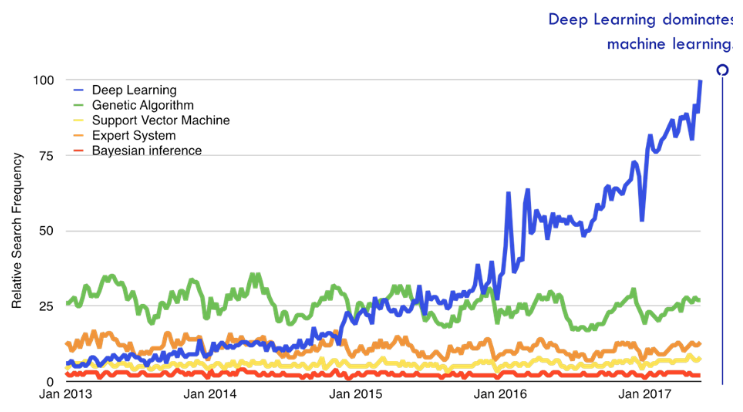
\includegraphics[scale=0.5]{images/deep-learning.png}
            \caption[The growth of deep learning compared to other machine learning algorithms]{The growth of deep learning compared to other machine learning algorithms \cite{leepdearning}}
            \label{fig:11}
        \end{figure}
        \par
        \par
        In the field Reinforcement Learning (RL), where tasks are learnt via trial-and-error by letting an agent
        interact with its environment, the same problem with handcrafted features exists. RL techniques rely on
        an internal representation of the state of the environment. This representation has to be derived from the
        agents percepts of the environment, which is most commonly done via handcrafted features. Therefore
        the applications of RL were limited to toy examples with a very low-dimensional state-space or to examples where the state-space could be thoroughly described via manually created features. Inspired by the
        advancements made in the field of deep learning, the subfield deep reinforcement learning emerged. As
        with deep learning in a supervised setting, a deep RL method also works directly on raw input instead
        of handcrafted features. Despite the young age of deep RL, several successful applications have already
        showed its power\cite{mnih2015humanlevel}\cite{DBLP:journals/corr/LevineFDA15}, among which AlphaGo is probably the best-known example \cite{deepGO}.
        \par
        This thesis will try to take even a step  further. While the vast majority of the newly developed deep
        RL methods were only tested on simple, basic simulations, it is reasonable to think that modern games, with complex strategies can also greatly benefit from deep RL techniques. However applying such methods
        involves many new challenges like e.g. dealing with huge state size and extremely long network convergence. This is exactly what is investigated
        in this thesis. More specifically the feasibility of the technique of Deep Q-Learning (DQL) \cite{mnih2015humanlevel} in complex and modern video games.

	\section{Problem Statement}
	    The main problem that will be discussed on this thesis is whether our new proposed method (Adam-DQL) is viable to solve complex video games. Specific research questions include:
        \begin{enumerate}
            \item How can the function that maps the in-game images into $Q$-values be determined?
            \item How can the desired function be represented?
            \item How viable is deep Q-learning to solve complex video games?
            \item Is it possible to improve techniques proposed by Deepmind using a better optimizer(Adam)?
            \item Is it possible to leverage the learning capabilities of Adam-DQL by adding policy improvement strategies such as partial training and demonstrations? 
    \end{enumerate}
        The secondary research questions are :
        \begin{enumerate}
            \item How can a general deep Q-learning implementation be developed ?
            \item What is the best structure of the software framework to allow seamless and efficient experiment? 
        \end{enumerate}
	    
%MODEL ASSUMPTIONS
	\section{Objectives}
	    The main objective of this thesis is to experimentally verify our method according to our problem statement. Listed below are the outline of our main objective in this thesis:
	    \begin{enumerate}
	    \item Develop a mathematical model, represented as directed acyclic graph, which maps a sequence of image to a vector of $Q$-values for each action. 
	    \item Develop a modified deep-Q learning technique using Adam optimizer.
        \item Develop a framework to allow an agent to interact with game environment.
        \item Implement the modified deep Q-learning for game environment.
        \item Describe and Interpret the results.
         \end{enumerate}
        To achieve the objectives described above, This thesis proposed several methods, which is listed below:
        \begin{enumerate}
        \item Review related research and literature.
        \item Develop a new deep learning algorithm, Adam-DQL, which consist of:
            \begin{enumerate}
            \item Modelling general video game as a Markov Decision Process.
            \item Deriving the Bellman optimality equation.
            \item Designing a neural network to approximate the $Q$-function.
            \item Deriving the loss function and gradient approximate equation.
            \item Implement a training algorithm for neural network based on DQN and Adam optimizer. 
            \item Address stability issues of Adam-DQL (partial training and demonstrations).
            \end{enumerate}
        
        \item Develop a software framework to interact with game environment, which consist of:
            \begin{enumerate}
            \item Implement Adam-DQL in Python.
            \item Modify and prepare few game environments to suit Adam-DQL testing requirements.
            \end{enumerate}
        
        \item Experimentally verify the capability of Adam-DQL, which consist of:
            \begin{enumerate}
            \item Train the neural network for a sample game.
            \item Describe and Interpret the Results.
            \end{enumerate}
        \end{enumerate}
        
   
		

	\section{Restrictions and Assumptions}
	    Since Adam-DQL is developed to create a general AI without any handcrafted features, Adam-DQL should work with every games, as long as it follows the restrictions and assumptions explained below:
        \begin{enumerate}
         \item The game environments are limited to the 1st stage only. This is more of a choice rather than a limitation. This choice comes from the fact that most games are designed to have an introductory stage, a stage that utilize every gameplay elements albeit being relatively simple. By restricting the scope to this introductory stages, the system can accommodate more gameplay concepts. Making the experiment much more accurate.
        \item Game environments can be stochastic. This assumption comes from the fact that generally, there's some random elements on games. Repeating the same action over and over again won't always produce the same result on these kind of games. By taking into account this stochastic elements, a more general, model-free method can be developed. 
        \item The Game has a constant amount of possible actions.
        This is a direct result of using output of a neural network to approximate the $Q$-function. A non constant amount of possible actions means the neural network has a non-constant output size. This is impossible since Neural networks structure is constant. An example of a game that doesn't have this constant action property is chess.
        \item The samples taken as minibatch in our training data are independent and identically distributed. This is the main requirement of using any stochastic/minibatch neural-network optimizer.
        \item The inputs for our neural network are taken from raw pixels and RAM(memory) only. This assumption allows the development of a system that is model-free, and can be used for general games with small to no modification.
        \item The interface layout for the game doesn't change overtime (static). Since adam-DQN's input is only raw pixels, it's not possible to accommodate a game that has changing game layout. Having a changing layout means the same position on the input might not represent the same thing overtime. This will create a noise in the training data and prevent the neural network to converge.
        \end{enumerate}
	
	\section{Benefits}
	There are several benefits of this research, both theoretical and practical, including:
	\subsection{Theoretical Benefits}
	\begin{enumerate}
	    
        \item
        Introduced new algorithm for higher-scale deep reinforcement learning in games. This will give an idea about how deep reinforcement learning with some modifications is highly usable in real world use case.
        \item Helps future researchers develop or compare various AIs by using software framework introduced in this thesis.
        \item A proof of concept that Demonstration, a technique used for robotics, can be applied to help solve complex games.
	    \item Introduced a new policy improvement technique called partial training, which kickstarts agent's reward for harder games.
	\end{enumerate}
	\subsection{Practical Benefits}
	\begin{enumerate}
        \item
        Allows the creation of general AI for more complex games, regardless of the genre and gameplay elements.
	\end{enumerate}

	\section{Thesis Structure}
	The writing structure of this thesis is as detailed below:
	\begin{enumerate}
	    \item Chapter I describes the background, problem statement, objectives, restrictions, and methodology. 
	    \item Chapter II describes the reinforcement learning with an emphasis on Q-learning and $\epsilon$-greedy policy. First, reinforcement learning in general will be presented, then, an introduction to reinforcement learning problem as Markov Decision Process will follow. After that, there will be some brief explanation about classical Q-learning algorithm and its feasibility in huge or immense state spaces. This chapter will be closed with an explanation of a classic problem in reinforcement learning, the exploration-exploitation dilemma. As well as $\epsilon$-greedy, an \textit{almost} greedy algorithm that solves the exploration-exploitation dilemma.
	    \item Chapter III describes the artificial neural networks, deep neural networks and deep learning technique. This chapter will start by explaining the underlying idea of artificial neural networks and convolutional neural networks. Then, it will be followed by the structural extension of artificial neural network, the deep neural networks. After that, there will be some quick introduction about how to train a neural network, as well as various optimizer (convex/nonconvex optimization algorithms). This chapter will be closed with an explanation of deep Q-learning, a method that combines reinforcement learning and deep neural networks.
	    \item Chapter IV contains implementation of deep Q-learning and the architecture of the whole learning system. This thesis propose a new modified algorithm called Adam-DQL that will be explained in this chapter. After that, the general structure of our framework will be described in detail. This chapter will also explain the structure of our neural network and every linearity (activation function) it uses. In this chapter we will also explain our state representation and our raw data input. 
	    \item Chapter V describes the various experiments and results for a sample game. This chapter will go even deeper into the selection of the framework architecture. There will be some experiment to test how well Adam-DQL performs in more modern games. However as explained earlier, Adam-DQL method should work for every game on the same platform with minimal to no changes. There will be some in-depth explanation about the results, as well as some comparison of Adam-DQL to other newly developed machine-learning algorithms.
	    \item Chapter VI summarizes achieved results, draw conclusions and proposes directions for further research.
	\end{enumerate}